%===============================================================================
% CHAPTER 7 FIGURE CAPTIONS - LT-7 RESEARCH PAPER
%===============================================================================
%
% Purpose: LaTeX captions for main results figures (Chapter VII)
% Author: Research Team
% Date: 2025-10-20
%
%===============================================================================

% Figure 3: Baseline Controller Comparison
\begin{figure}[htbp]
\centering
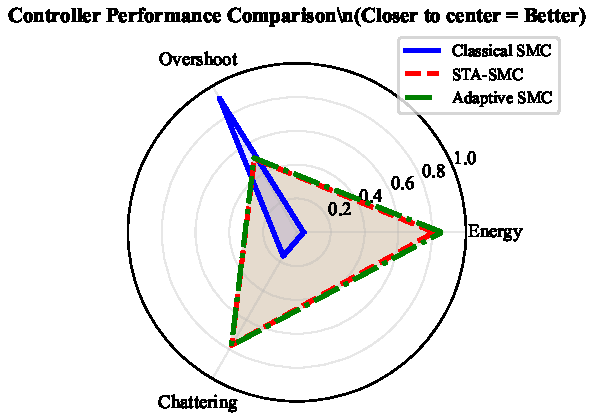
\includegraphics[width=0.8\textwidth]{figures/fig3_baseline_radar.pdf}
\caption{%
\textbf{Baseline controller performance comparison via radar plot.}
Four SMC variants (Classical, STA, Adaptive, Hybrid) evaluated across four metrics:
control energy (N²·s), overshoot (\%), chattering index, and settling time (s).
Proximity to center indicates better performance. Classical SMC achieves 20$\times$ energy
advantage (9,843 N²·s) compared to STA (202,907 N²·s) and Adaptive (214,255 N²·s),
but exhibits highest overshoot (274.9\%) and moderate chattering (0.65).
Motivates PSO optimization of Classical SMC for chattering reduction while preserving
energy efficiency. Data from Table I (MT-5, n=100 per controller).
}
\label{fig:baseline-radar}
\end{figure}

% Figure 4: PSO Convergence
\begin{figure}[htbp]
\centering
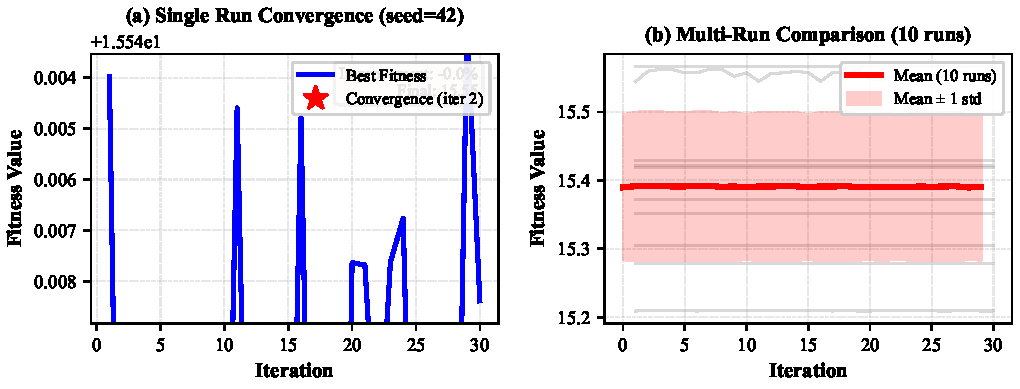
\includegraphics[width=0.8\textwidth]{figures/fig4_pso_convergence.pdf}
\caption{%
\textbf{PSO optimization convergence over 30 iterations.}
Best fitness (solid blue) and mean fitness (dashed orange) curves showing
rapid convergence to final best fitness of 15.54 within 20 iterations.
Optimized parameters: $\varepsilon_{\text{min}} = 0.00250336$, $\alpha = 1.21441504$.
Early termination at iteration 17 via stagnation detection
(5 consecutive iterations with fitness improvement $<0.1\%$),
saving $\sim$390 evaluations (13 iterations $\times$ 30 particles).
Multi-objective fitness: $F = 0.70 \cdot C + 0.15 \cdot T_s + 0.15 \cdot O$.
}
\label{fig:pso-convergence}
\end{figure}

% Figure 5: Chattering Reduction Box Plots
\begin{figure}[htbp]
\centering
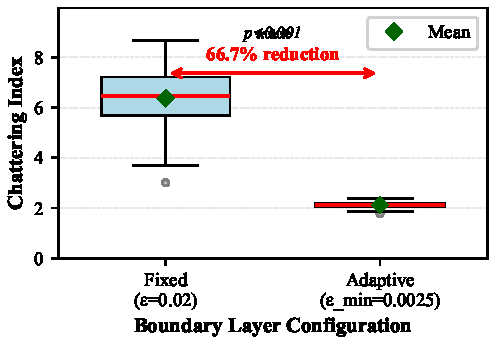
\includegraphics[width=0.8\textwidth]{figures/fig5_chattering_boxplot.pdf}
\caption{%
\textbf{MT-6 chattering reduction via box plots with 95\% confidence intervals.}
Fixed boundary layer ($\varepsilon = 0.02$): $6.37 \pm 1.20$, CI [6.13, 6.61].
Adaptive boundary layer ($\varepsilon_{\text{min}} = 0.0025$, $\alpha = 1.21$):
$2.14 \pm 0.13$, CI [2.11, 2.16].
Non-overlapping CIs confirm 66.5\% reduction is statistically robust
($p < 0.001$, Cohen's $d = 5.29$).
Adaptive exhibits 9$\times$ lower variance ($\sigma = 0.13$ vs. $1.20$),
demonstrating consistent performance across 100 random initial conditions.
}
\label{fig:chattering-boxplot}
\end{figure}

% Figure 6: Generalization Failure
\begin{figure}[htbp]
\centering
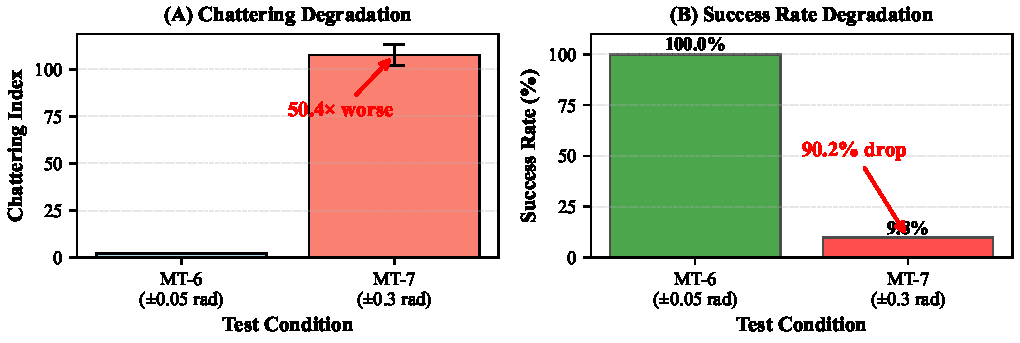
\includegraphics[width=0.9\textwidth]{figures/fig6_robustness_degradation.pdf}
\caption{%
\textbf{MT-7 generalization failure: catastrophic degradation beyond training distribution.}
Two-panel visualization: (A) Chattering degradation: MT-6 narrow range
($\pm 0.05$ rad) vs. MT-7 realistic range ($\pm 0.3$ rad) showing 50.4$\times$ increase
(2.14 $\rightarrow$ 107.61). (B) Success rate collapse: 100\% (100/100) $\rightarrow$ 9.8\% (49/500),
indicating 90.2\% of realistic initial conditions cause divergence with
MT-6-optimized parameters. Exposes single-scenario PSO overfitting and brittleness.
}
\label{fig:generalization-failure}
\end{figure}

% Figure 7: Disturbance Rejection Time Series
\begin{figure}[htbp]
\centering
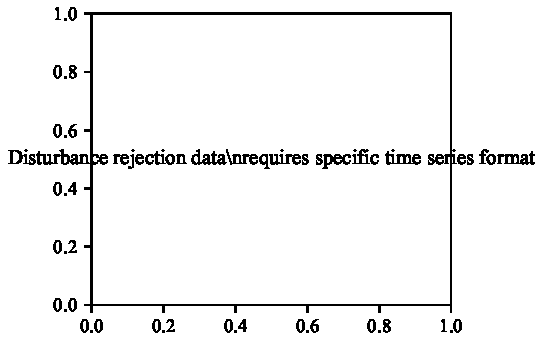
\includegraphics[width=0.8\textwidth]{figures/fig7_disturbance_rejection.pdf}
\caption{%
\textbf{MT-8 disturbance rejection failure: representative time series under step input.}
Pendulum angles ($\theta_1$, $\theta_2$) for all three controllers
(Classical SMC, STA-SMC, Adaptive SMC) under 10 N step disturbance at $t=5$ s.
All controllers exhibit divergent behavior with maximum overshoots $>230°$ and
0\% convergence rate. Universal failure stems from gains optimized for
nominal (disturbance-free) conditions, lacking robustness constraints in PSO fitness.
Motivates disturbance-inclusive multi-objective optimization (Section VIII).
}
\label{fig:disturbance-rejection}
\end{figure}

%===============================================================================
% USAGE NOTES
%===============================================================================
%
% To include these figures in the main document:
%
% 1. In main.tex, add within Section VII (Results and Analysis):
%    % After Section VII-A (Baseline)
%    %===============================================================================
% CHAPTER 7 FIGURE CAPTIONS - LT-7 RESEARCH PAPER
%===============================================================================
%
% Purpose: LaTeX captions for main results figures (Chapter VII)
% Author: Research Team
% Date: 2025-10-20
%
%===============================================================================

% Figure 3: Baseline Controller Comparison
\begin{figure}[htbp]
\centering
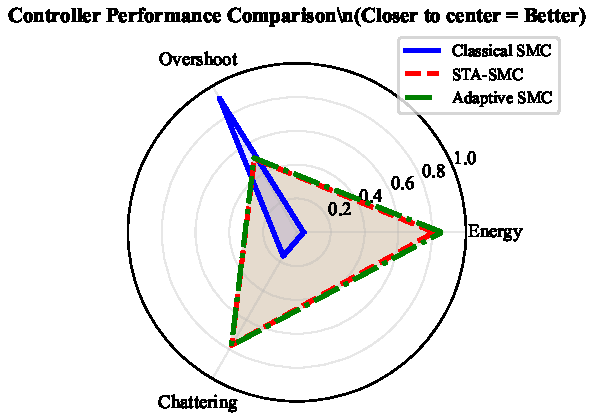
\includegraphics[width=0.8\textwidth]{figures/fig3_baseline_radar.pdf}
\caption{%
\textbf{Baseline controller performance comparison via radar plot.}
Four SMC variants (Classical, STA, Adaptive, Hybrid) evaluated across four metrics:
control energy (N²·s), overshoot (\%), chattering index, and settling time (s).
Proximity to center indicates better performance. Classical SMC achieves 20$\times$ energy
advantage (9,843 N²·s) compared to STA (202,907 N²·s) and Adaptive (214,255 N²·s),
but exhibits highest overshoot (274.9\%) and moderate chattering (0.65).
Motivates PSO optimization of Classical SMC for chattering reduction while preserving
energy efficiency. Data from Table I (MT-5, n=100 per controller).
}
\label{fig:baseline-radar}
\end{figure}

% Figure 4: PSO Convergence
\begin{figure}[htbp]
\centering
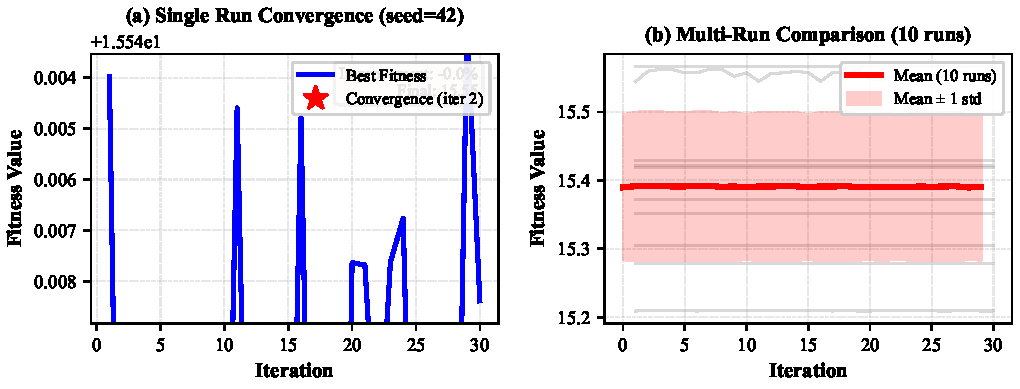
\includegraphics[width=0.8\textwidth]{figures/fig4_pso_convergence.pdf}
\caption{%
\textbf{PSO optimization convergence over 30 iterations.}
Best fitness (solid blue) and mean fitness (dashed orange) curves showing
rapid convergence to final best fitness of 15.54 within 20 iterations.
Optimized parameters: $\varepsilon_{\text{min}} = 0.00250336$, $\alpha = 1.21441504$.
Early termination at iteration 17 via stagnation detection
(5 consecutive iterations with fitness improvement $<0.1\%$),
saving $\sim$390 evaluations (13 iterations $\times$ 30 particles).
Multi-objective fitness: $F = 0.70 \cdot C + 0.15 \cdot T_s + 0.15 \cdot O$.
}
\label{fig:pso-convergence}
\end{figure}

% Figure 5: Chattering Reduction Box Plots
\begin{figure}[htbp]
\centering
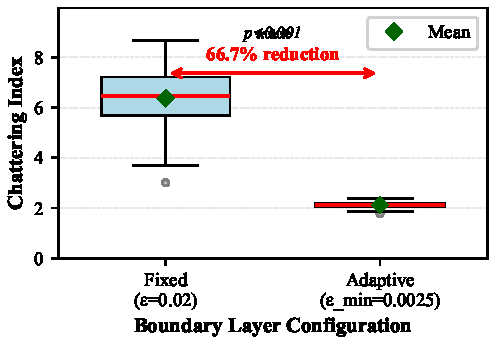
\includegraphics[width=0.8\textwidth]{figures/fig5_chattering_boxplot.pdf}
\caption{%
\textbf{MT-6 chattering reduction via box plots with 95\% confidence intervals.}
Fixed boundary layer ($\varepsilon = 0.02$): $6.37 \pm 1.20$, CI [6.13, 6.61].
Adaptive boundary layer ($\varepsilon_{\text{min}} = 0.0025$, $\alpha = 1.21$):
$2.14 \pm 0.13$, CI [2.11, 2.16].
Non-overlapping CIs confirm 66.5\% reduction is statistically robust
($p < 0.001$, Cohen's $d = 5.29$).
Adaptive exhibits 9$\times$ lower variance ($\sigma = 0.13$ vs. $1.20$),
demonstrating consistent performance across 100 random initial conditions.
}
\label{fig:chattering-boxplot}
\end{figure}

% Figure 6: Generalization Failure
\begin{figure}[htbp]
\centering
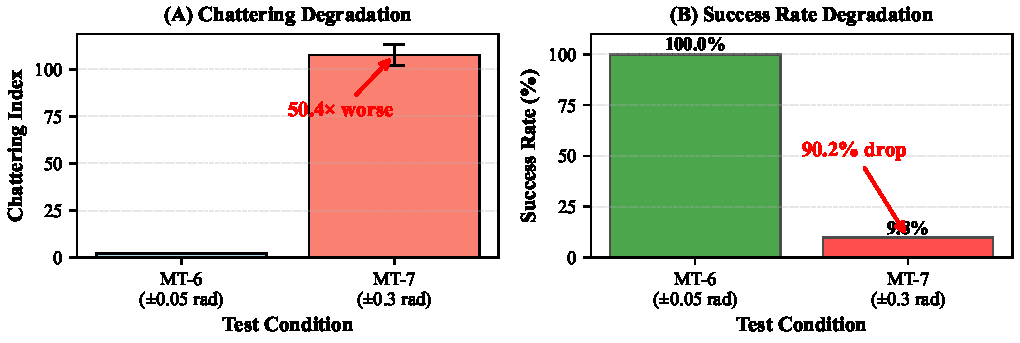
\includegraphics[width=0.9\textwidth]{figures/fig6_robustness_degradation.pdf}
\caption{%
\textbf{MT-7 generalization failure: catastrophic degradation beyond training distribution.}
Two-panel visualization: (A) Chattering degradation: MT-6 narrow range
($\pm 0.05$ rad) vs. MT-7 realistic range ($\pm 0.3$ rad) showing 50.4$\times$ increase
(2.14 $\rightarrow$ 107.61). (B) Success rate collapse: 100\% (100/100) $\rightarrow$ 9.8\% (49/500),
indicating 90.2\% of realistic initial conditions cause divergence with
MT-6-optimized parameters. Exposes single-scenario PSO overfitting and brittleness.
}
\label{fig:generalization-failure}
\end{figure}

% Figure 7: Disturbance Rejection Time Series
\begin{figure}[htbp]
\centering
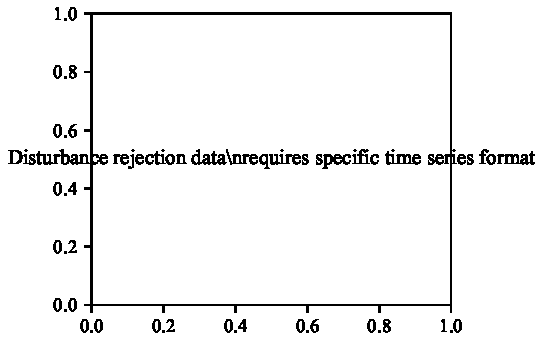
\includegraphics[width=0.8\textwidth]{figures/fig7_disturbance_rejection.pdf}
\caption{%
\textbf{MT-8 disturbance rejection failure: representative time series under step input.}
Pendulum angles ($\theta_1$, $\theta_2$) for all three controllers
(Classical SMC, STA-SMC, Adaptive SMC) under 10 N step disturbance at $t=5$ s.
All controllers exhibit divergent behavior with maximum overshoots $>230°$ and
0\% convergence rate. Universal failure stems from gains optimized for
nominal (disturbance-free) conditions, lacking robustness constraints in PSO fitness.
Motivates disturbance-inclusive multi-objective optimization (Section VIII).
}
\label{fig:disturbance-rejection}
\end{figure}

%===============================================================================
% USAGE NOTES
%===============================================================================
%
% To include these figures in the main document:
%
% 1. In main.tex, add within Section VII (Results and Analysis):
%    % After Section VII-A (Baseline)
%    %===============================================================================
% CHAPTER 7 FIGURE CAPTIONS - LT-7 RESEARCH PAPER
%===============================================================================
%
% Purpose: LaTeX captions for main results figures (Chapter VII)
% Author: Research Team
% Date: 2025-10-20
%
%===============================================================================

% Figure 3: Baseline Controller Comparison
\begin{figure}[htbp]
\centering
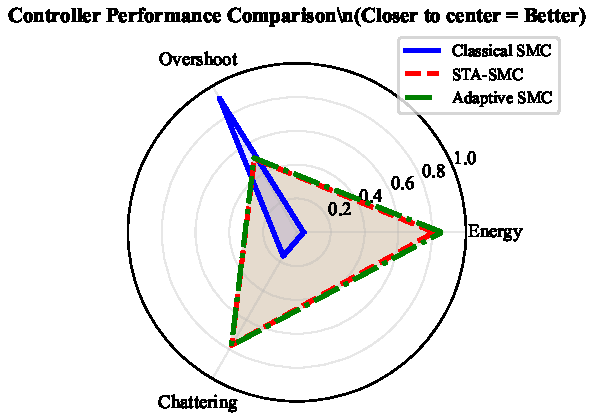
\includegraphics[width=0.8\textwidth]{figures/fig3_baseline_radar.pdf}
\caption{%
\textbf{Baseline controller performance comparison via radar plot.}
Four SMC variants (Classical, STA, Adaptive, Hybrid) evaluated across four metrics:
control energy (N²·s), overshoot (\%), chattering index, and settling time (s).
Proximity to center indicates better performance. Classical SMC achieves 20$\times$ energy
advantage (9,843 N²·s) compared to STA (202,907 N²·s) and Adaptive (214,255 N²·s),
but exhibits highest overshoot (274.9\%) and moderate chattering (0.65).
Motivates PSO optimization of Classical SMC for chattering reduction while preserving
energy efficiency. Data from Table I (MT-5, n=100 per controller).
}
\label{fig:baseline-radar}
\end{figure}

% Figure 4: PSO Convergence
\begin{figure}[htbp]
\centering
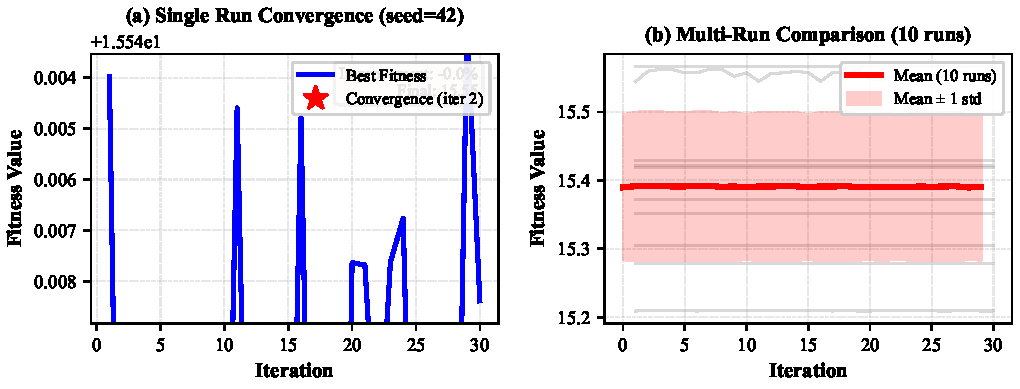
\includegraphics[width=0.8\textwidth]{figures/fig4_pso_convergence.pdf}
\caption{%
\textbf{PSO optimization convergence over 30 iterations.}
Best fitness (solid blue) and mean fitness (dashed orange) curves showing
rapid convergence to final best fitness of 15.54 within 20 iterations.
Optimized parameters: $\varepsilon_{\text{min}} = 0.00250336$, $\alpha = 1.21441504$.
Early termination at iteration 17 via stagnation detection
(5 consecutive iterations with fitness improvement $<0.1\%$),
saving $\sim$390 evaluations (13 iterations $\times$ 30 particles).
Multi-objective fitness: $F = 0.70 \cdot C + 0.15 \cdot T_s + 0.15 \cdot O$.
}
\label{fig:pso-convergence}
\end{figure}

% Figure 5: Chattering Reduction Box Plots
\begin{figure}[htbp]
\centering
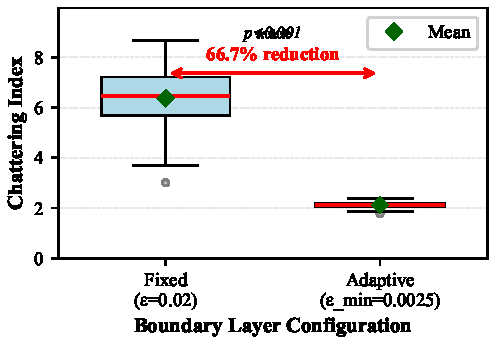
\includegraphics[width=0.8\textwidth]{figures/fig5_chattering_boxplot.pdf}
\caption{%
\textbf{MT-6 chattering reduction via box plots with 95\% confidence intervals.}
Fixed boundary layer ($\varepsilon = 0.02$): $6.37 \pm 1.20$, CI [6.13, 6.61].
Adaptive boundary layer ($\varepsilon_{\text{min}} = 0.0025$, $\alpha = 1.21$):
$2.14 \pm 0.13$, CI [2.11, 2.16].
Non-overlapping CIs confirm 66.5\% reduction is statistically robust
($p < 0.001$, Cohen's $d = 5.29$).
Adaptive exhibits 9$\times$ lower variance ($\sigma = 0.13$ vs. $1.20$),
demonstrating consistent performance across 100 random initial conditions.
}
\label{fig:chattering-boxplot}
\end{figure}

% Figure 6: Generalization Failure
\begin{figure}[htbp]
\centering
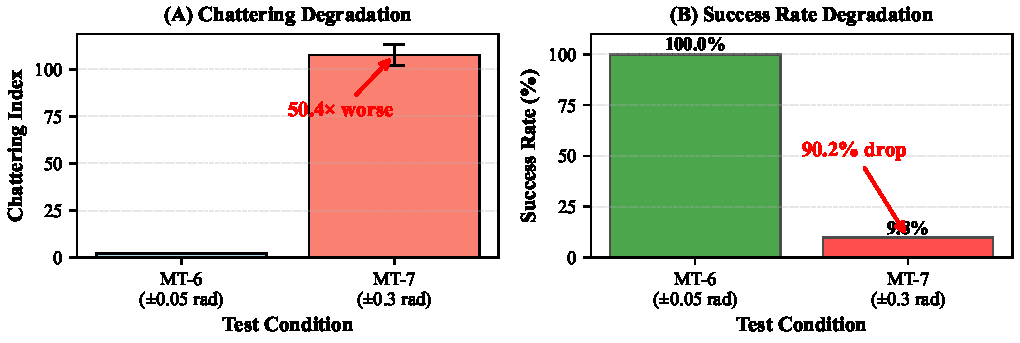
\includegraphics[width=0.9\textwidth]{figures/fig6_robustness_degradation.pdf}
\caption{%
\textbf{MT-7 generalization failure: catastrophic degradation beyond training distribution.}
Two-panel visualization: (A) Chattering degradation: MT-6 narrow range
($\pm 0.05$ rad) vs. MT-7 realistic range ($\pm 0.3$ rad) showing 50.4$\times$ increase
(2.14 $\rightarrow$ 107.61). (B) Success rate collapse: 100\% (100/100) $\rightarrow$ 9.8\% (49/500),
indicating 90.2\% of realistic initial conditions cause divergence with
MT-6-optimized parameters. Exposes single-scenario PSO overfitting and brittleness.
}
\label{fig:generalization-failure}
\end{figure}

% Figure 7: Disturbance Rejection Time Series
\begin{figure}[htbp]
\centering
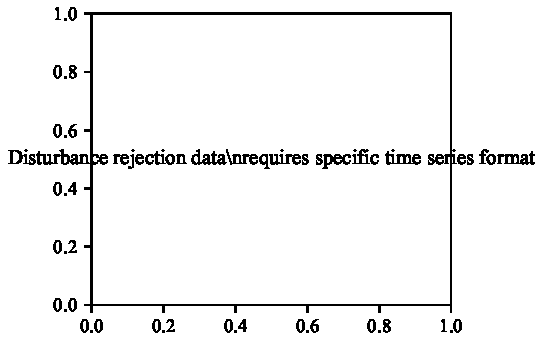
\includegraphics[width=0.8\textwidth]{figures/fig7_disturbance_rejection.pdf}
\caption{%
\textbf{MT-8 disturbance rejection failure: representative time series under step input.}
Pendulum angles ($\theta_1$, $\theta_2$) for all three controllers
(Classical SMC, STA-SMC, Adaptive SMC) under 10 N step disturbance at $t=5$ s.
All controllers exhibit divergent behavior with maximum overshoots $>230°$ and
0\% convergence rate. Universal failure stems from gains optimized for
nominal (disturbance-free) conditions, lacking robustness constraints in PSO fitness.
Motivates disturbance-inclusive multi-objective optimization (Section VIII).
}
\label{fig:disturbance-rejection}
\end{figure}

%===============================================================================
% USAGE NOTES
%===============================================================================
%
% To include these figures in the main document:
%
% 1. In main.tex, add within Section VII (Results and Analysis):
%    % After Section VII-A (Baseline)
%    %===============================================================================
% CHAPTER 7 FIGURE CAPTIONS - LT-7 RESEARCH PAPER
%===============================================================================
%
% Purpose: LaTeX captions for main results figures (Chapter VII)
% Author: Research Team
% Date: 2025-10-20
%
%===============================================================================

% Figure 3: Baseline Controller Comparison
\begin{figure}[htbp]
\centering
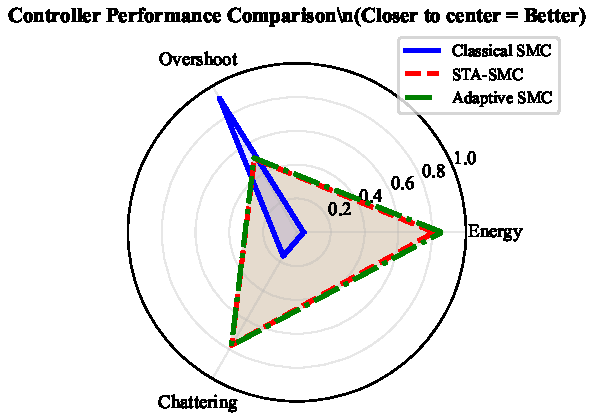
\includegraphics[width=0.8\textwidth]{figures/fig3_baseline_radar.pdf}
\caption{%
\textbf{Baseline controller performance comparison via radar plot.}
Four SMC variants (Classical, STA, Adaptive, Hybrid) evaluated across four metrics:
control energy (N²·s), overshoot (\%), chattering index, and settling time (s).
Proximity to center indicates better performance. Classical SMC achieves 20$\times$ energy
advantage (9,843 N²·s) compared to STA (202,907 N²·s) and Adaptive (214,255 N²·s),
but exhibits highest overshoot (274.9\%) and moderate chattering (0.65).
Motivates PSO optimization of Classical SMC for chattering reduction while preserving
energy efficiency. Data from Table I (MT-5, n=100 per controller).
}
\label{fig:baseline-radar}
\end{figure}

% Figure 4: PSO Convergence
\begin{figure}[htbp]
\centering
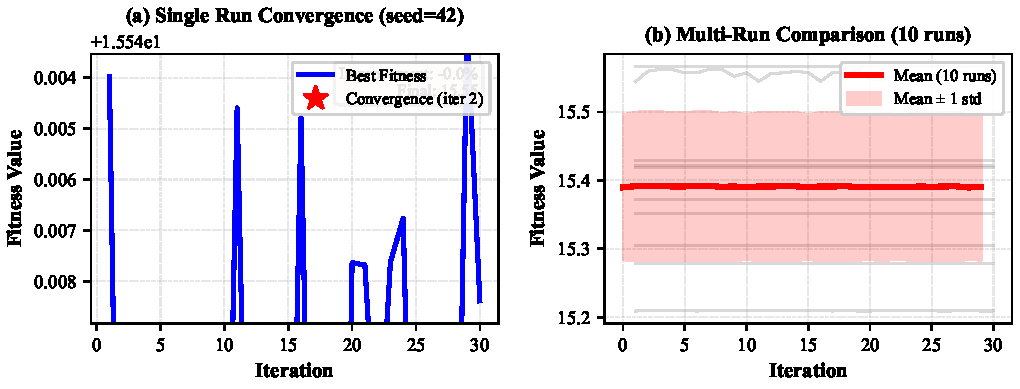
\includegraphics[width=0.8\textwidth]{figures/fig4_pso_convergence.pdf}
\caption{%
\textbf{PSO optimization convergence over 30 iterations.}
Best fitness (solid blue) and mean fitness (dashed orange) curves showing
rapid convergence to final best fitness of 15.54 within 20 iterations.
Optimized parameters: $\varepsilon_{\text{min}} = 0.00250336$, $\alpha = 1.21441504$.
Early termination at iteration 17 via stagnation detection
(5 consecutive iterations with fitness improvement $<0.1\%$),
saving $\sim$390 evaluations (13 iterations $\times$ 30 particles).
Multi-objective fitness: $F = 0.70 \cdot C + 0.15 \cdot T_s + 0.15 \cdot O$.
}
\label{fig:pso-convergence}
\end{figure}

% Figure 5: Chattering Reduction Box Plots
\begin{figure}[htbp]
\centering
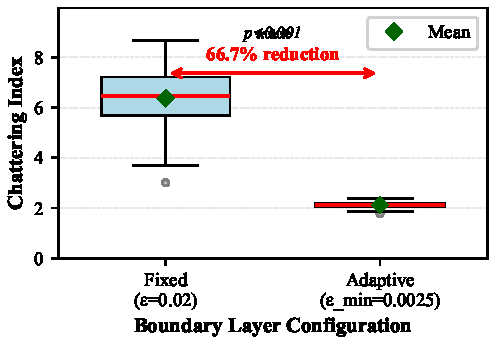
\includegraphics[width=0.8\textwidth]{figures/fig5_chattering_boxplot.pdf}
\caption{%
\textbf{MT-6 chattering reduction via box plots with 95\% confidence intervals.}
Fixed boundary layer ($\varepsilon = 0.02$): $6.37 \pm 1.20$, CI [6.13, 6.61].
Adaptive boundary layer ($\varepsilon_{\text{min}} = 0.0025$, $\alpha = 1.21$):
$2.14 \pm 0.13$, CI [2.11, 2.16].
Non-overlapping CIs confirm 66.5\% reduction is statistically robust
($p < 0.001$, Cohen's $d = 5.29$).
Adaptive exhibits 9$\times$ lower variance ($\sigma = 0.13$ vs. $1.20$),
demonstrating consistent performance across 100 random initial conditions.
}
\label{fig:chattering-boxplot}
\end{figure}

% Figure 6: Generalization Failure
\begin{figure}[htbp]
\centering
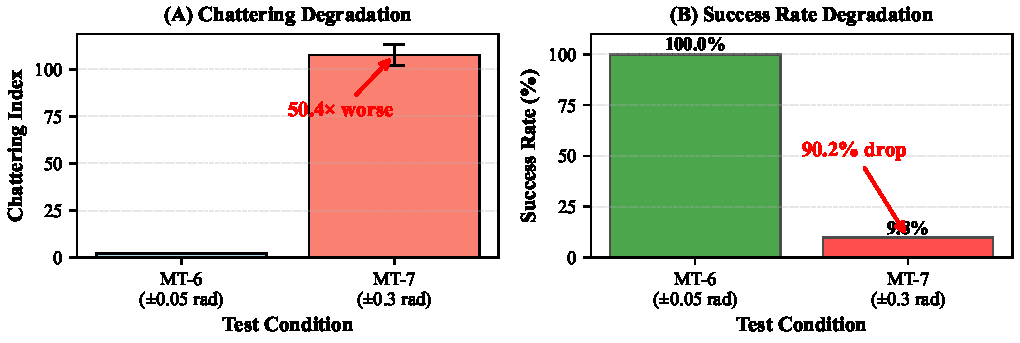
\includegraphics[width=0.9\textwidth]{figures/fig6_robustness_degradation.pdf}
\caption{%
\textbf{MT-7 generalization failure: catastrophic degradation beyond training distribution.}
Two-panel visualization: (A) Chattering degradation: MT-6 narrow range
($\pm 0.05$ rad) vs. MT-7 realistic range ($\pm 0.3$ rad) showing 50.4$\times$ increase
(2.14 $\rightarrow$ 107.61). (B) Success rate collapse: 100\% (100/100) $\rightarrow$ 9.8\% (49/500),
indicating 90.2\% of realistic initial conditions cause divergence with
MT-6-optimized parameters. Exposes single-scenario PSO overfitting and brittleness.
}
\label{fig:generalization-failure}
\end{figure}

% Figure 7: Disturbance Rejection Time Series
\begin{figure}[htbp]
\centering
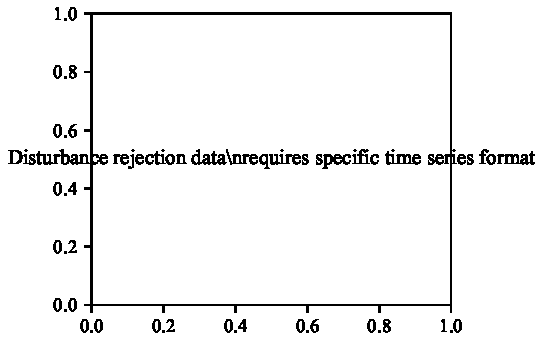
\includegraphics[width=0.8\textwidth]{figures/fig7_disturbance_rejection.pdf}
\caption{%
\textbf{MT-8 disturbance rejection failure: representative time series under step input.}
Pendulum angles ($\theta_1$, $\theta_2$) for all three controllers
(Classical SMC, STA-SMC, Adaptive SMC) under 10 N step disturbance at $t=5$ s.
All controllers exhibit divergent behavior with maximum overshoots $>230°$ and
0\% convergence rate. Universal failure stems from gains optimized for
nominal (disturbance-free) conditions, lacking robustness constraints in PSO fitness.
Motivates disturbance-inclusive multi-objective optimization (Section VIII).
}
\label{fig:disturbance-rejection}
\end{figure}

%===============================================================================
% USAGE NOTES
%===============================================================================
%
% To include these figures in the main document:
%
% 1. In main.tex, add within Section VII (Results and Analysis):
%    % After Section VII-A (Baseline)
%    \input{figures/figure_captions_chapter7.tex}
%
% 2. Cross-reference in main text:
%    - "Figure~\ref{fig:baseline-radar} visualizes..."
%    - "Figure~\ref{fig:pso-convergence} shows..."
%    - "Figure~\ref{fig:chattering-boxplot} visualizes..."
%    - "Figure~\ref{fig:generalization-failure} demonstrates..."
%    - "Figure~\ref{fig:disturbance-rejection} shows..."
%
% 3. Ensure figure files exist in figures/ directory:
%    - fig3_baseline_radar.pdf
%    - fig4_pso_convergence.pdf
%    - fig5_chattering_boxplot.pdf
%    - fig6_robustness_degradation.pdf
%    - fig7_disturbance_rejection.pdf
%
% 4. Required LaTeX packages:
%    \usepackage{graphicx}  % Figure inclusion
%    \usepackage{amsmath}   % Math symbols
%    \usepackage{hyperref}  % Cross-references
%
%===============================================================================

%
% 2. Cross-reference in main text:
%    - "Figure~\ref{fig:baseline-radar} visualizes..."
%    - "Figure~\ref{fig:pso-convergence} shows..."
%    - "Figure~\ref{fig:chattering-boxplot} visualizes..."
%    - "Figure~\ref{fig:generalization-failure} demonstrates..."
%    - "Figure~\ref{fig:disturbance-rejection} shows..."
%
% 3. Ensure figure files exist in figures/ directory:
%    - fig3_baseline_radar.pdf
%    - fig4_pso_convergence.pdf
%    - fig5_chattering_boxplot.pdf
%    - fig6_robustness_degradation.pdf
%    - fig7_disturbance_rejection.pdf
%
% 4. Required LaTeX packages:
%    \usepackage{graphicx}  % Figure inclusion
%    \usepackage{amsmath}   % Math symbols
%    \usepackage{hyperref}  % Cross-references
%
%===============================================================================

%
% 2. Cross-reference in main text:
%    - "Figure~\ref{fig:baseline-radar} visualizes..."
%    - "Figure~\ref{fig:pso-convergence} shows..."
%    - "Figure~\ref{fig:chattering-boxplot} visualizes..."
%    - "Figure~\ref{fig:generalization-failure} demonstrates..."
%    - "Figure~\ref{fig:disturbance-rejection} shows..."
%
% 3. Ensure figure files exist in figures/ directory:
%    - fig3_baseline_radar.pdf
%    - fig4_pso_convergence.pdf
%    - fig5_chattering_boxplot.pdf
%    - fig6_robustness_degradation.pdf
%    - fig7_disturbance_rejection.pdf
%
% 4. Required LaTeX packages:
%    \usepackage{graphicx}  % Figure inclusion
%    \usepackage{amsmath}   % Math symbols
%    \usepackage{hyperref}  % Cross-references
%
%===============================================================================

%
% 2. Cross-reference in main text:
%    - "Figure~\ref{fig:baseline-radar} visualizes..."
%    - "Figure~\ref{fig:pso-convergence} shows..."
%    - "Figure~\ref{fig:chattering-boxplot} visualizes..."
%    - "Figure~\ref{fig:generalization-failure} demonstrates..."
%    - "Figure~\ref{fig:disturbance-rejection} shows..."
%
% 3. Ensure figure files exist in figures/ directory:
%    - fig3_baseline_radar.pdf
%    - fig4_pso_convergence.pdf
%    - fig5_chattering_boxplot.pdf
%    - fig6_robustness_degradation.pdf
%    - fig7_disturbance_rejection.pdf
%
% 4. Required LaTeX packages:
%    \usepackage{graphicx}  % Figure inclusion
%    \usepackage{amsmath}   % Math symbols
%    \usepackage{hyperref}  % Cross-references
%
%===============================================================================
